FlexPMS er opbygget af adskillige tråde, som alle kan snakke sammen ved at sende beskeder til hinanden. Trådene håndterer udelukkende beskeder sendt til dem udefra, og står derfor udelukkende i blokerende kald til en besked-kø, så længe de ikke er ved at håndtere en indkommende besked. Trådene nedarver fra \textit{MessageThread} og har pointers til de tråde, som de skal kunne sende beskeder til.

\SekvensDiagram{0.82}{FlexPMS}{FlexPMS}

\KlasseDiagram{0.82}{FlexPMS}{FlexPMS}

\subsubsection{MessageThread}
Klassen, som er en specialisering af \textit{Thread}, stiller funktionalitet til rådighed til at indgå i det event-baserede beskedsystem. Ved at nedarve fra \textit{MessageThread} bliver en klasse til en modtager af beskeder, og kan i den forbindelse nøjes med at implementere en \textKode{dispatch()} metode, som kaldes hver gang tråden modtager en besked via dens send() metode. \textKode{dispatch()} modtager to argumenter; et event-ID samt en pointer til et \textit{Message}-objekt, der evt. kan være \textKode{NULL}. Dispatch bør overholde reglen om, at kalde en funktion til at håndtere beskeden alt efter hvilket event-ID den modtager.\\\\

\textKode{send()} tager ligeledes to argumenter; et event-ID samt en pointer til et \textit{Message}-objekt. Det er afsenderen, som skal allokere \textit{Message}-objektet, men \textit{MessageThread} sørger selv for, at de-allokere det efter \textKode{dispatch()} er kaldt hos modtageren.\\\\

\textit{MessageThread} laver udelukkende blokerende kald til dens besked-kø, og dermed undgår vi, at stå og bruge CPU-tid i løkker, som ikke udfører noget. Det betyder, at alle klasse som nedarver fra \textit{MessageThread} udelukkende håndterer events sendt til dem udefra. På den måde lægges tråde til at sove så længe der ikke er noget at lave, og programmet vil bruge minimalt CPU-tid.


\StateDiagram{0.82}{FlexPMS}{Template}

\subsubsection{Arkitekturspecifikke metoder}

\funk{virtual void init()}{Abstrakt metode, som kaldes inden der begyndes at hente beskeder fra beskedkøen}{Ingenting}
{}

\funk{void send(unsigned long id, Message* msg = NULL)}{Lægger en besked i trådens beskedkø}{Ingenting}
{
\funkArg{id}{Et ID, som beskriver det event der sendes}
\funkArg{msg}{En pointer til et Message-objekt, som kan holde på yderligere data}
}

\funk{virtual void dispatch(unsigned long event\_id, Message* msg))}{Abstrakt metode, som kaldes hver gang tråden modtager en besked. Metoden skal overskrives af klasser, som nedarver fra MessageThread til at håndtere indkommende beskeder}{Ingenting}
{
\funkArg{event\_id}{Et ID, som beskriver det event der sendes}
\funkArg{msg}{En pointer til et Message-objekt, som kan holde på yderligere data. Kan være \textKode{NULL}}
}


\subsubsection{MessageQueue}

Klassen er en FIFO kø, som er trådsikret, dvs. sikret mod de problemer der kan opstå i forbindelse med at tilgå den parallelt fra forskellige tråde. \textit{MessageQueue} er implementeret via en queue (fra STL) og benytter sig at pthread’s \textit{mutex} og \textit{conditional variable} til at synkronisere mellem tråde. \textit{MessageQueue} er udelukkende brugt internt i \textit{MessageThread}.

\begin{figure}[H]
	\centering
	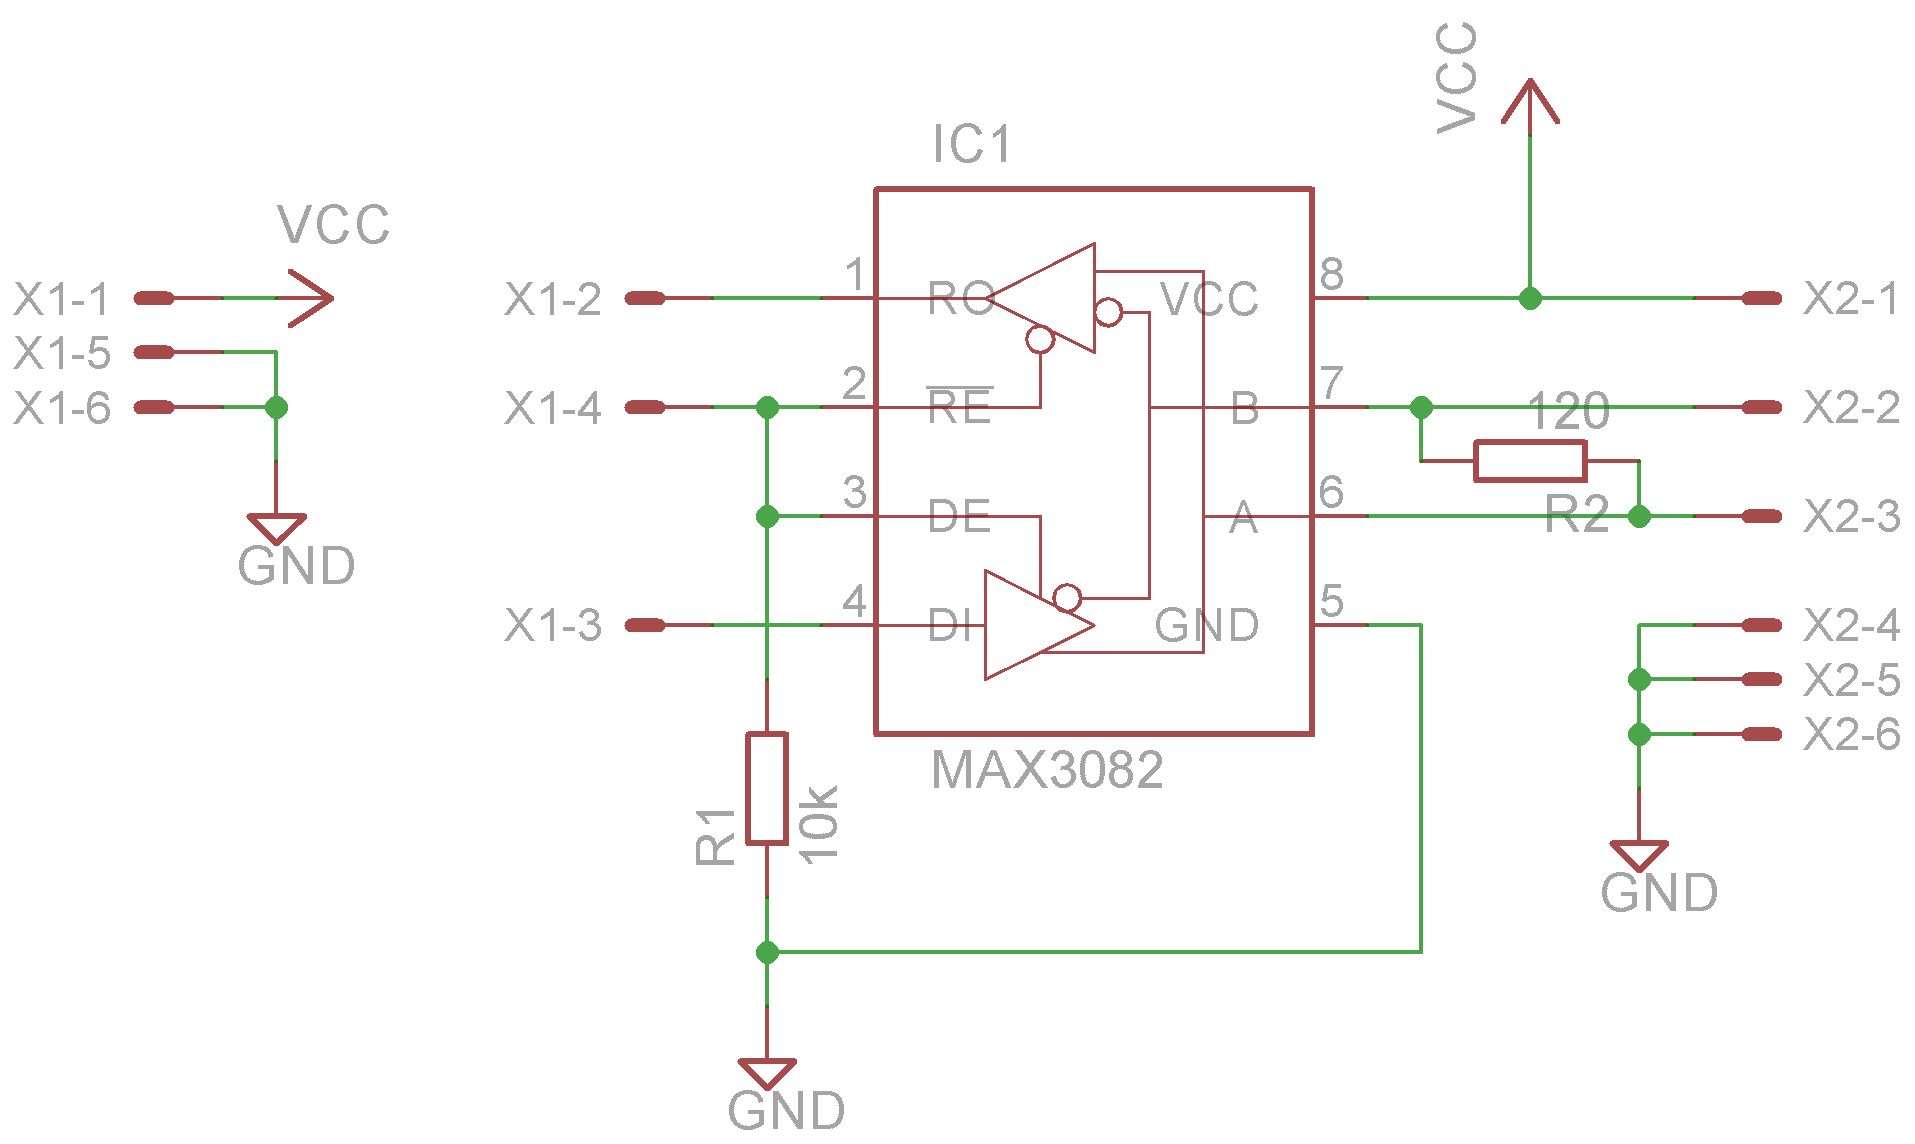
\includegraphics[scale=1]{../Hardware/RS485_Converter/Schematic}
	\caption{RS485 converter}
	\label{photo:RS485converter}
\end{figure}